\documentclass[12pt,]{article}
\usepackage{lmodern}
\usepackage{amssymb,amsmath}
\usepackage{ifxetex,ifluatex}
\usepackage{fixltx2e} % provides \textsubscript
\ifnum 0\ifxetex 1\fi\ifluatex 1\fi=0 % if pdftex
  \usepackage[T1]{fontenc}
  \usepackage[utf8]{inputenc}
\else % if luatex or xelatex
  \ifxetex
    \usepackage{mathspec}
  \else
    \usepackage{fontspec}
  \fi
  \defaultfontfeatures{Ligatures=TeX,Scale=MatchLowercase}
    \setmainfont[]{Arial}
\fi
% use upquote if available, for straight quotes in verbatim environments
\IfFileExists{upquote.sty}{\usepackage{upquote}}{}
% use microtype if available
\IfFileExists{microtype.sty}{%
\usepackage{microtype}
\UseMicrotypeSet[protrusion]{basicmath} % disable protrusion for tt fonts
}{}
\usepackage[margin=1in]{geometry}
\usepackage{hyperref}
\PassOptionsToPackage{usenames,dvipsnames}{color} % color is loaded by hyperref
\hypersetup{unicode=true,
            pdftitle={Supervised learning: Regression 2},
            colorlinks=true,
            linkcolor=Maroon,
            citecolor=Blue,
            urlcolor=blue,
            breaklinks=true}
\urlstyle{same}  % don't use monospace font for urls
\usepackage{color}
\usepackage{fancyvrb}
\newcommand{\VerbBar}{|}
\newcommand{\VERB}{\Verb[commandchars=\\\{\}]}
\DefineVerbatimEnvironment{Highlighting}{Verbatim}{commandchars=\\\{\}}
% Add ',fontsize=\small' for more characters per line
\usepackage{framed}
\definecolor{shadecolor}{RGB}{248,248,248}
\newenvironment{Shaded}{\begin{snugshade}}{\end{snugshade}}
\newcommand{\AlertTok}[1]{\textcolor[rgb]{0.94,0.16,0.16}{#1}}
\newcommand{\AnnotationTok}[1]{\textcolor[rgb]{0.56,0.35,0.01}{\textbf{\textit{#1}}}}
\newcommand{\AttributeTok}[1]{\textcolor[rgb]{0.77,0.63,0.00}{#1}}
\newcommand{\BaseNTok}[1]{\textcolor[rgb]{0.00,0.00,0.81}{#1}}
\newcommand{\BuiltInTok}[1]{#1}
\newcommand{\CharTok}[1]{\textcolor[rgb]{0.31,0.60,0.02}{#1}}
\newcommand{\CommentTok}[1]{\textcolor[rgb]{0.56,0.35,0.01}{\textit{#1}}}
\newcommand{\CommentVarTok}[1]{\textcolor[rgb]{0.56,0.35,0.01}{\textbf{\textit{#1}}}}
\newcommand{\ConstantTok}[1]{\textcolor[rgb]{0.00,0.00,0.00}{#1}}
\newcommand{\ControlFlowTok}[1]{\textcolor[rgb]{0.13,0.29,0.53}{\textbf{#1}}}
\newcommand{\DataTypeTok}[1]{\textcolor[rgb]{0.13,0.29,0.53}{#1}}
\newcommand{\DecValTok}[1]{\textcolor[rgb]{0.00,0.00,0.81}{#1}}
\newcommand{\DocumentationTok}[1]{\textcolor[rgb]{0.56,0.35,0.01}{\textbf{\textit{#1}}}}
\newcommand{\ErrorTok}[1]{\textcolor[rgb]{0.64,0.00,0.00}{\textbf{#1}}}
\newcommand{\ExtensionTok}[1]{#1}
\newcommand{\FloatTok}[1]{\textcolor[rgb]{0.00,0.00,0.81}{#1}}
\newcommand{\FunctionTok}[1]{\textcolor[rgb]{0.00,0.00,0.00}{#1}}
\newcommand{\ImportTok}[1]{#1}
\newcommand{\InformationTok}[1]{\textcolor[rgb]{0.56,0.35,0.01}{\textbf{\textit{#1}}}}
\newcommand{\KeywordTok}[1]{\textcolor[rgb]{0.13,0.29,0.53}{\textbf{#1}}}
\newcommand{\NormalTok}[1]{#1}
\newcommand{\OperatorTok}[1]{\textcolor[rgb]{0.81,0.36,0.00}{\textbf{#1}}}
\newcommand{\OtherTok}[1]{\textcolor[rgb]{0.56,0.35,0.01}{#1}}
\newcommand{\PreprocessorTok}[1]{\textcolor[rgb]{0.56,0.35,0.01}{\textit{#1}}}
\newcommand{\RegionMarkerTok}[1]{#1}
\newcommand{\SpecialCharTok}[1]{\textcolor[rgb]{0.00,0.00,0.00}{#1}}
\newcommand{\SpecialStringTok}[1]{\textcolor[rgb]{0.31,0.60,0.02}{#1}}
\newcommand{\StringTok}[1]{\textcolor[rgb]{0.31,0.60,0.02}{#1}}
\newcommand{\VariableTok}[1]{\textcolor[rgb]{0.00,0.00,0.00}{#1}}
\newcommand{\VerbatimStringTok}[1]{\textcolor[rgb]{0.31,0.60,0.02}{#1}}
\newcommand{\WarningTok}[1]{\textcolor[rgb]{0.56,0.35,0.01}{\textbf{\textit{#1}}}}
\usepackage{graphicx,grffile}
\makeatletter
\def\maxwidth{\ifdim\Gin@nat@width>\linewidth\linewidth\else\Gin@nat@width\fi}
\def\maxheight{\ifdim\Gin@nat@height>\textheight\textheight\else\Gin@nat@height\fi}
\makeatother
% Scale images if necessary, so that they will not overflow the page
% margins by default, and it is still possible to overwrite the defaults
% using explicit options in \includegraphics[width, height, ...]{}
\setkeys{Gin}{width=\maxwidth,height=\maxheight,keepaspectratio}
\IfFileExists{parskip.sty}{%
\usepackage{parskip}
}{% else
\setlength{\parindent}{0pt}
\setlength{\parskip}{6pt plus 2pt minus 1pt}
}
\setlength{\emergencystretch}{3em}  % prevent overfull lines
\providecommand{\tightlist}{%
  \setlength{\itemsep}{0pt}\setlength{\parskip}{0pt}}
\setcounter{secnumdepth}{0}
% Redefines (sub)paragraphs to behave more like sections
\ifx\paragraph\undefined\else
\let\oldparagraph\paragraph
\renewcommand{\paragraph}[1]{\oldparagraph{#1}\mbox{}}
\fi
\ifx\subparagraph\undefined\else
\let\oldsubparagraph\subparagraph
\renewcommand{\subparagraph}[1]{\oldsubparagraph{#1}\mbox{}}
\fi

%%% Use protect on footnotes to avoid problems with footnotes in titles
\let\rmarkdownfootnote\footnote%
\def\footnote{\protect\rmarkdownfootnote}

%%% Change title format to be more compact
\usepackage{titling}

% Create subtitle command for use in maketitle
\newcommand{\subtitle}[1]{
  \posttitle{
    \begin{center}\large#1\end{center}
    }
}

\setlength{\droptitle}{-2em}

  \title{Supervised learning: Regression 2}
    \pretitle{\vspace{\droptitle}\centering\huge}
  \posttitle{\par}
    \author{}
    \preauthor{}\postauthor{}
    \date{}
    \predate{}\postdate{}
  

\begin{document}
\maketitle

{
\hypersetup{linkcolor=black}
\setcounter{tocdepth}{1}
\tableofcontents
}
\hypertarget{introduction}{%
\section{Introduction}\label{introduction}}

In this practical, you will learn how to handle many variables with
regression by using variable selection techniques, and how to tune
hyperparameters for these techniques. This practical has been derived
from chapter 6 of ISLR.

One of the packages we are going to use is \texttt{glmnet}. For this,
you will probably need to \texttt{install.packages("glmnet")} before
running the \texttt{library()} functions.

\begin{Shaded}
\begin{Highlighting}[]
\KeywordTok{library}\NormalTok{(ISLR)}
\KeywordTok{library}\NormalTok{(glmnet)}
\KeywordTok{library}\NormalTok{(tidyverse)}
\end{Highlighting}
\end{Shaded}

\hypertarget{best-subset-selection}{%
\section{Best subset selection}\label{best-subset-selection}}

Our goal for today is to use the \texttt{Hitters} dataset from the
\texttt{ISLR} package to predict \texttt{Salary}.

\begin{center}\rule{0.5\linewidth}{\linethickness}\end{center}

\textbf{Prepare a dataframe \texttt{baseball} from the Hitters dataset
but without the baseball players for which the \texttt{Salary} is
missing. How many baseball players are left?}

\begin{center}\rule{0.5\linewidth}{\linethickness}\end{center}

\begin{Shaded}
\begin{Highlighting}[]
\NormalTok{baseball <-}\StringTok{ }\NormalTok{Hitters }\OperatorTok\StringTok{ }\KeywordTok{filter}\NormalTok{(}\OperatorTok{!}\KeywordTok{is.na}\NormalTok{(Salary))}

\KeywordTok{nrow}\NormalTok{(baseball)}
\end{Highlighting}
\end{Shaded}

\begin{verbatim}
## [1] 263
\end{verbatim}

\begin{center}\rule{0.5\linewidth}{\linethickness}\end{center}

\textbf{Create \texttt{baseball\_train} (50\%), \texttt{baseball\_valid}
(30\%), and \texttt{baseball\_test} (20\%) datasets.}

\begin{center}\rule{0.5\linewidth}{\linethickness}\end{center}

\begin{Shaded}
\begin{Highlighting}[]
\NormalTok{split <-}\StringTok{ }\KeywordTok{c}\NormalTok{(}\KeywordTok{rep}\NormalTok{(}\StringTok{"train"}\NormalTok{, }\DecValTok{132}\NormalTok{), }\KeywordTok{rep}\NormalTok{(}\StringTok{"valid"}\NormalTok{, }\DecValTok{79}\NormalTok{), }\KeywordTok{rep}\NormalTok{(}\StringTok{"test"}\NormalTok{,  }\DecValTok{52}\NormalTok{))}
\NormalTok{baseball <-}\StringTok{ }\NormalTok{baseball }\OperatorTok\StringTok{ }\KeywordTok{mutate}\NormalTok{(}\DataTypeTok{split =} \KeywordTok{sample}\NormalTok{(split))}

\NormalTok{baseball_train <-}\StringTok{ }\NormalTok{baseball }\OperatorTok\StringTok{ }\KeywordTok{filter}\NormalTok{(split }\OperatorTok{==}\StringTok{ "train"}\NormalTok{)}
\NormalTok{baseball_valid <-}\StringTok{ }\NormalTok{baseball }\OperatorTok\StringTok{ }\KeywordTok{filter}\NormalTok{(split }\OperatorTok{==}\StringTok{ "valid"}\NormalTok{)}
\NormalTok{baseball_test  <-}\StringTok{ }\NormalTok{baseball }\OperatorTok\StringTok{ }\KeywordTok{filter}\NormalTok{(split }\OperatorTok{==}\StringTok{ "test"}\NormalTok{)}
\end{Highlighting}
\end{Shaded}

\begin{center}\rule{0.5\linewidth}{\linethickness}\end{center}

\textbf{Create a function called \texttt{lm\_mse()} with as input a
formula and a training dataset and a test dataset which outputs the mse
on the test dataset for predictions from a linear model.}

\begin{center}\rule{0.5\linewidth}{\linethickness}\end{center}

Start like this:

\begin{Shaded}
\begin{Highlighting}[]
\NormalTok{mse <-}\StringTok{ }\ControlFlowTok{function}\NormalTok{(y_true, y_pred) }\KeywordTok{sum}\NormalTok{((y_true }\OperatorTok{-}\StringTok{ }\NormalTok{y_pred)}\OperatorTok{^}\DecValTok{2}\NormalTok{)}

\NormalTok{lm_mse <-}\StringTok{ }\ControlFlowTok{function}\NormalTok{(formula, train_data, valid_data) \{}
\NormalTok{  y_name <-}\StringTok{ }\KeywordTok{as.character}\NormalTok{(formula)[}\DecValTok{2}\NormalTok{]}
\NormalTok{  y_true <-}\StringTok{ }\NormalTok{valid_data[[y_name]]}
  
  \CommentTok{# The remainder of the function here}
\NormalTok{\}}
\end{Highlighting}
\end{Shaded}

\begin{Shaded}
\begin{Highlighting}[]
\NormalTok{mse <-}\StringTok{ }\ControlFlowTok{function}\NormalTok{(y_true, y_pred) }\KeywordTok{sum}\NormalTok{((y_true }\OperatorTok{-}\StringTok{ }\NormalTok{y_pred)}\OperatorTok{^}\DecValTok{2}\NormalTok{)}

\NormalTok{lm_mse <-}\StringTok{ }\ControlFlowTok{function}\NormalTok{(formula, train_data, valid_data) \{}
\NormalTok{  y_name <-}\StringTok{ }\KeywordTok{as.character}\NormalTok{(formula)[}\DecValTok{2}\NormalTok{]}
\NormalTok{  y_true <-}\StringTok{ }\NormalTok{valid_data[[y_name]]}
  
\NormalTok{  lm_fit <-}\StringTok{ }\KeywordTok{lm}\NormalTok{(formula, train_data)}
\NormalTok{  y_pred <-}\StringTok{ }\KeywordTok{predict}\NormalTok{(lm_fit, }\DataTypeTok{newdata =}\NormalTok{ valid_data)}
  
  \KeywordTok{mse}\NormalTok{(y_true, y_pred)}
\NormalTok{\}}
\end{Highlighting}
\end{Shaded}

\begin{center}\rule{0.5\linewidth}{\linethickness}\end{center}

\textbf{Try out your function with the formula
\texttt{Salary\ \textasciitilde{}\ Hits\ +\ Runs}, using
\texttt{baseball\_train} and \texttt{baseball\_valid}.}

\begin{center}\rule{0.5\linewidth}{\linethickness}\end{center}

\begin{Shaded}
\begin{Highlighting}[]
\KeywordTok{lm_mse}\NormalTok{(Salary }\OperatorTok{~}\StringTok{ }\NormalTok{Hits }\OperatorTok{+}\StringTok{ }\NormalTok{Runs, baseball_train, baseball_valid)}
\end{Highlighting}
\end{Shaded}

\begin{verbatim}
## [1] 14443687
\end{verbatim}

\begin{Shaded}
\begin{Highlighting}[]
\KeywordTok{lm_mse}\NormalTok{(Salary }\OperatorTok{~}\StringTok{ }\NormalTok{Hits, baseball_train, baseball_valid)}
\end{Highlighting}
\end{Shaded}

\begin{verbatim}
## [1] 14347232
\end{verbatim}

We have pre-programmed a function for you to output \emph{all} formulas
with \texttt{p} variables as characters You can load the function into
your environment by \emph{sourcing} the \texttt{.R} file it is written
in:

\begin{Shaded}
\begin{Highlighting}[]
\KeywordTok{source}\NormalTok{(}\StringTok{"generate_formulas.R"}\NormalTok{)}
\end{Highlighting}
\end{Shaded}

You can use it like so:

\begin{Shaded}
\begin{Highlighting}[]
\KeywordTok{generate_formulas}\NormalTok{(}\DataTypeTok{p =} \DecValTok{2}\NormalTok{, }\DataTypeTok{x_vars =} \KeywordTok{c}\NormalTok{(}\StringTok{"x1"}\NormalTok{, }\StringTok{"x2"}\NormalTok{, }\StringTok{"x3"}\NormalTok{, }\StringTok{"x4"}\NormalTok{), }\DataTypeTok{y_var =} \StringTok{"y"}\NormalTok{)}
\end{Highlighting}
\end{Shaded}

\begin{verbatim}
## [1] "y ~ x1 + x2" "y ~ x1 + x3" "y ~ x1 + x4" "y ~ x2 + x3" "y ~ x2 + x4"
## [6] "y ~ x3 + x4"
\end{verbatim}

\begin{center}\rule{0.5\linewidth}{\linethickness}\end{center}

\textbf{Create a character vector of all predictor variables from the
\texttt{Hitters} dataset. \texttt{colnames()} may be of help. Note that
\texttt{Salary} is not a predictor variable}

\begin{center}\rule{0.5\linewidth}{\linethickness}\end{center}

\begin{Shaded}
\begin{Highlighting}[]
\NormalTok{x_vars <-}\StringTok{ }\KeywordTok{colnames}\NormalTok{(Hitters)}
\NormalTok{x_vars <-}\StringTok{ }\NormalTok{x_vars[x_vars }\OperatorTok{!=}\StringTok{ "Salary"}\NormalTok{]}
\end{Highlighting}
\end{Shaded}

\begin{center}\rule{0.5\linewidth}{\linethickness}\end{center}

\textbf{Generate all formulas with as outcome \texttt{Salary} and 3
predictors from the \texttt{Hitters} data. Assign this to a variable
called \texttt{formulas}. There should be \$\choose{19}{3} = \$ 969
elements in this vector.}

\begin{center}\rule{0.5\linewidth}{\linethickness}\end{center}

\begin{Shaded}
\begin{Highlighting}[]
\NormalTok{formulas <-}\StringTok{ }\KeywordTok{generate_formulas}\NormalTok{(}\DataTypeTok{p =} \DecValTok{3}\NormalTok{, }\DataTypeTok{x_vars =}\NormalTok{ x_vars, }\DataTypeTok{y_var =} \StringTok{"Salary"}\NormalTok{)}
\KeywordTok{length}\NormalTok{(formulas)}
\end{Highlighting}
\end{Shaded}

\begin{verbatim}
## [1] 969
\end{verbatim}

\begin{center}\rule{0.5\linewidth}{\linethickness}\end{center}

\textbf{Use a \texttt{for\ loop} to find the best set of 3 predictors in
the \texttt{Hitters} dataset based on MSE. Use the
\texttt{baseball\_train} and \texttt{baseball\_valid} datasets.}

\begin{center}\rule{0.5\linewidth}{\linethickness}\end{center}

\begin{Shaded}
\begin{Highlighting}[]
\CommentTok{# Initialise a vector we will fill with MSE values}
\NormalTok{mses <-}\StringTok{ }\KeywordTok{rep}\NormalTok{(}\DecValTok{0}\NormalTok{, }\DecValTok{969}\NormalTok{)}

\CommentTok{# loop over all the formulas}
\ControlFlowTok{for}\NormalTok{ (i }\ControlFlowTok{in} \DecValTok{1}\OperatorTok{:}\DecValTok{969}\NormalTok{) \{}
\NormalTok{  mses[i] <-}\StringTok{ }\KeywordTok{lm_mse}\NormalTok{(}\KeywordTok{as.formula}\NormalTok{(formulas[i]), baseball_train, baseball_valid)}
\NormalTok{\}}

\CommentTok{# select the formula with the lowest MSE}
\NormalTok{best_}\DecValTok{3}\NormalTok{_preds <-}\StringTok{ }\NormalTok{formulas[}\KeywordTok{which.min}\NormalTok{(mses)]}
\end{Highlighting}
\end{Shaded}

\begin{center}\rule{0.5\linewidth}{\linethickness}\end{center}

\textbf{Do the same for 1, 2 and 4 predictors. Now select the best model
with 1, 2, 3, or 4 predictors in terms of its out-of-sample MSE}

\begin{center}\rule{0.5\linewidth}{\linethickness}\end{center}

\begin{Shaded}
\begin{Highlighting}[]
\CommentTok{# Generate formulas}
\NormalTok{formulas_}\DecValTok{1}\NormalTok{ <-}\StringTok{ }\KeywordTok{generate_formulas}\NormalTok{(}\DataTypeTok{p =} \DecValTok{1}\NormalTok{, }\DataTypeTok{x_vars =}\NormalTok{ x_vars, }\DataTypeTok{y_var =} \StringTok{"Salary"}\NormalTok{)}
\NormalTok{formulas_}\DecValTok{2}\NormalTok{ <-}\StringTok{ }\KeywordTok{generate_formulas}\NormalTok{(}\DataTypeTok{p =} \DecValTok{2}\NormalTok{, }\DataTypeTok{x_vars =}\NormalTok{ x_vars, }\DataTypeTok{y_var =} \StringTok{"Salary"}\NormalTok{)}
\NormalTok{formulas_}\DecValTok{4}\NormalTok{ <-}\StringTok{ }\KeywordTok{generate_formulas}\NormalTok{(}\DataTypeTok{p =} \DecValTok{4}\NormalTok{, }\DataTypeTok{x_vars =}\NormalTok{ x_vars, }\DataTypeTok{y_var =} \StringTok{"Salary"}\NormalTok{)}

\CommentTok{# Initialise a vector we will fill with MSE values}
\NormalTok{mses_}\DecValTok{1}\NormalTok{ <-}\StringTok{ }\KeywordTok{rep}\NormalTok{(}\DecValTok{0}\NormalTok{, }\KeywordTok{length}\NormalTok{(formulas_}\DecValTok{1}\NormalTok{))}
\NormalTok{mses_}\DecValTok{2}\NormalTok{ <-}\StringTok{ }\KeywordTok{rep}\NormalTok{(}\DecValTok{0}\NormalTok{, }\KeywordTok{length}\NormalTok{(formulas_}\DecValTok{2}\NormalTok{))}
\NormalTok{mses_}\DecValTok{4}\NormalTok{ <-}\StringTok{ }\KeywordTok{rep}\NormalTok{(}\DecValTok{0}\NormalTok{, }\KeywordTok{length}\NormalTok{(formulas_}\DecValTok{4}\NormalTok{))}

\CommentTok{# loop over all the formulas}
\ControlFlowTok{for}\NormalTok{ (i }\ControlFlowTok{in} \DecValTok{1}\OperatorTok{:}\KeywordTok{length}\NormalTok{(formulas_}\DecValTok{1}\NormalTok{)) \{}
\NormalTok{  mses_}\DecValTok{1}\NormalTok{[i] <-}\StringTok{ }\KeywordTok{lm_mse}\NormalTok{(}\KeywordTok{as.formula}\NormalTok{(formulas_}\DecValTok{1}\NormalTok{[i]), baseball_train, baseball_valid)}
\NormalTok{\}}

\ControlFlowTok{for}\NormalTok{ (i }\ControlFlowTok{in} \DecValTok{1}\OperatorTok{:}\KeywordTok{length}\NormalTok{(formulas_}\DecValTok{2}\NormalTok{)) \{}
\NormalTok{  mses_}\DecValTok{2}\NormalTok{[i] <-}\StringTok{ }\KeywordTok{lm_mse}\NormalTok{(}\KeywordTok{as.formula}\NormalTok{(formulas_}\DecValTok{2}\NormalTok{[i]), baseball_train, baseball_valid)}
\NormalTok{\}}

\ControlFlowTok{for}\NormalTok{ (i }\ControlFlowTok{in} \DecValTok{1}\OperatorTok{:}\KeywordTok{length}\NormalTok{(formulas_}\DecValTok{4}\NormalTok{)) \{}
\NormalTok{  mses_}\DecValTok{4}\NormalTok{[i] <-}\StringTok{ }\KeywordTok{lm_mse}\NormalTok{(}\KeywordTok{as.formula}\NormalTok{(formulas_}\DecValTok{4}\NormalTok{[i]), baseball_train, baseball_valid)}
\NormalTok{\}}

\CommentTok{# Compare mses}
\KeywordTok{min}\NormalTok{(mses_}\DecValTok{1}\NormalTok{)}
\KeywordTok{min}\NormalTok{(mses_}\DecValTok{2}\NormalTok{)}
\KeywordTok{min}\NormalTok{(mses)}
\KeywordTok{min}\NormalTok{(mses_}\DecValTok{4}\NormalTok{)}

\CommentTok{# min(mses_4) is lowest of them all!}
\CommentTok{# So let's see which model that is}

\NormalTok{formulas_}\DecValTok{4}\NormalTok{[}\KeywordTok{which.min}\NormalTok{(mses_}\DecValTok{4}\NormalTok{)]}
\end{Highlighting}
\end{Shaded}

\begin{verbatim}
## [1] 10819945
## [1] 9482279
## [1] 8815829
## [1] 8310934
## [1] "Salary ~ Walks + CAtBat + CHits + CRBI"
\end{verbatim}

\begin{center}\rule{0.5\linewidth}{\linethickness}\end{center}

\textbf{Calculate the test MSE for this model. Then, create a plot
comparing predicted values (mapped to x position) versus observed values
(mapped to y position) of \texttt{baseball\_test}.}

\begin{center}\rule{0.5\linewidth}{\linethickness}\end{center}

\begin{Shaded}
\begin{Highlighting}[]
\CommentTok{# Estimate model and calculate mse}
\NormalTok{lm_best <-}\StringTok{ }\KeywordTok{lm}\NormalTok{(Salary }\OperatorTok{~}\StringTok{ }\NormalTok{Runs }\OperatorTok{+}\StringTok{ }\NormalTok{CHits }\OperatorTok{+}\StringTok{ }\NormalTok{Division }\OperatorTok{+}\StringTok{ }\NormalTok{PutOuts, baseball_train)}
\KeywordTok{mse}\NormalTok{(baseball_test}\OperatorTok{$}\NormalTok{Salary, }\KeywordTok{predict}\NormalTok{(lm_best, }\DataTypeTok{newdata =}\NormalTok{ baseball_test))}
\end{Highlighting}
\end{Shaded}

\begin{verbatim}
## [1] 6182329
\end{verbatim}

\begin{Shaded}
\begin{Highlighting}[]
\CommentTok{# create a plot}
\KeywordTok{tibble}\NormalTok{(}
  \DataTypeTok{y_true =}\NormalTok{ baseball_test}\OperatorTok{$}\NormalTok{Salary,}
  \DataTypeTok{y_pred =} \KeywordTok{predict}\NormalTok{(lm_best, }\DataTypeTok{newdata =}\NormalTok{ baseball_test)}
\NormalTok{) }\OperatorTok\StringTok{ }
\StringTok{  }\KeywordTok{ggplot}\NormalTok{(}\KeywordTok{aes}\NormalTok{(}\DataTypeTok{x =}\NormalTok{ y_pred, }\DataTypeTok{y =}\NormalTok{ y_true)) }\OperatorTok{+}
\StringTok{  }\KeywordTok{geom_abline}\NormalTok{(}\DataTypeTok{slope =} \DecValTok{1}\NormalTok{, }\DataTypeTok{intercept =} \DecValTok{0}\NormalTok{, }\DataTypeTok{lty =} \DecValTok{2}\NormalTok{) }\OperatorTok{+}
\StringTok{  }\KeywordTok{geom_point}\NormalTok{() }\OperatorTok{+}
\StringTok{  }\KeywordTok{theme_minimal}\NormalTok{()}
\end{Highlighting}
\end{Shaded}

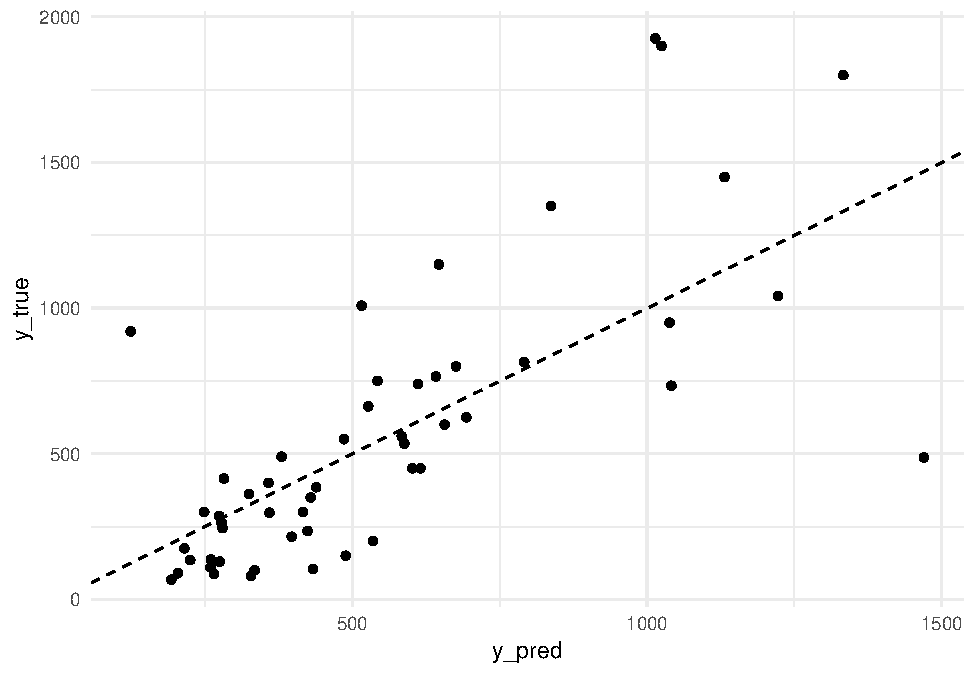
\includegraphics{regression_2_files/figure-latex/msefinal-1.pdf}


\end{document}
